\documentclass{standalone}
\usepackage{ tikz }
\usepackage{ xparse }
\usepackage{../../../macros}

\begin{document}
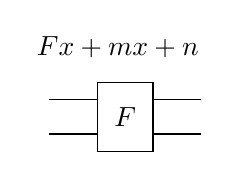
\begin{tikzpicture}[yscale=-1,x=1em,y=1.25em]

    \node at (3,-1) {$\morph{F}{x + m}{x + n}$};

    \draw (0.5,0.5) -- (2.25,0.5); 
    \draw (0.5,1.5) -- (2.25,1.5);

    \draw (4.25,0.5) -- (6,0.5);
    \draw (4.25,1.5) -- (6,1.5);
    
    \node[draw, minimum height = 2.5em, minimum width = 2em, anchor = west] at (2.25,1){$F$};
\end{tikzpicture}
\end{document}